% Figure 3: Multi-Scale Resonance Shell Hierarchy
% Concentric shells from quantum to global scale with phi-ratio radii
\documentclass[tikz,border=5pt]{standalone}
\usepackage{tikz}
\usetikzlibrary{calc,decorations.pathmorphing,arrows.meta,patterns}

\begin{document}
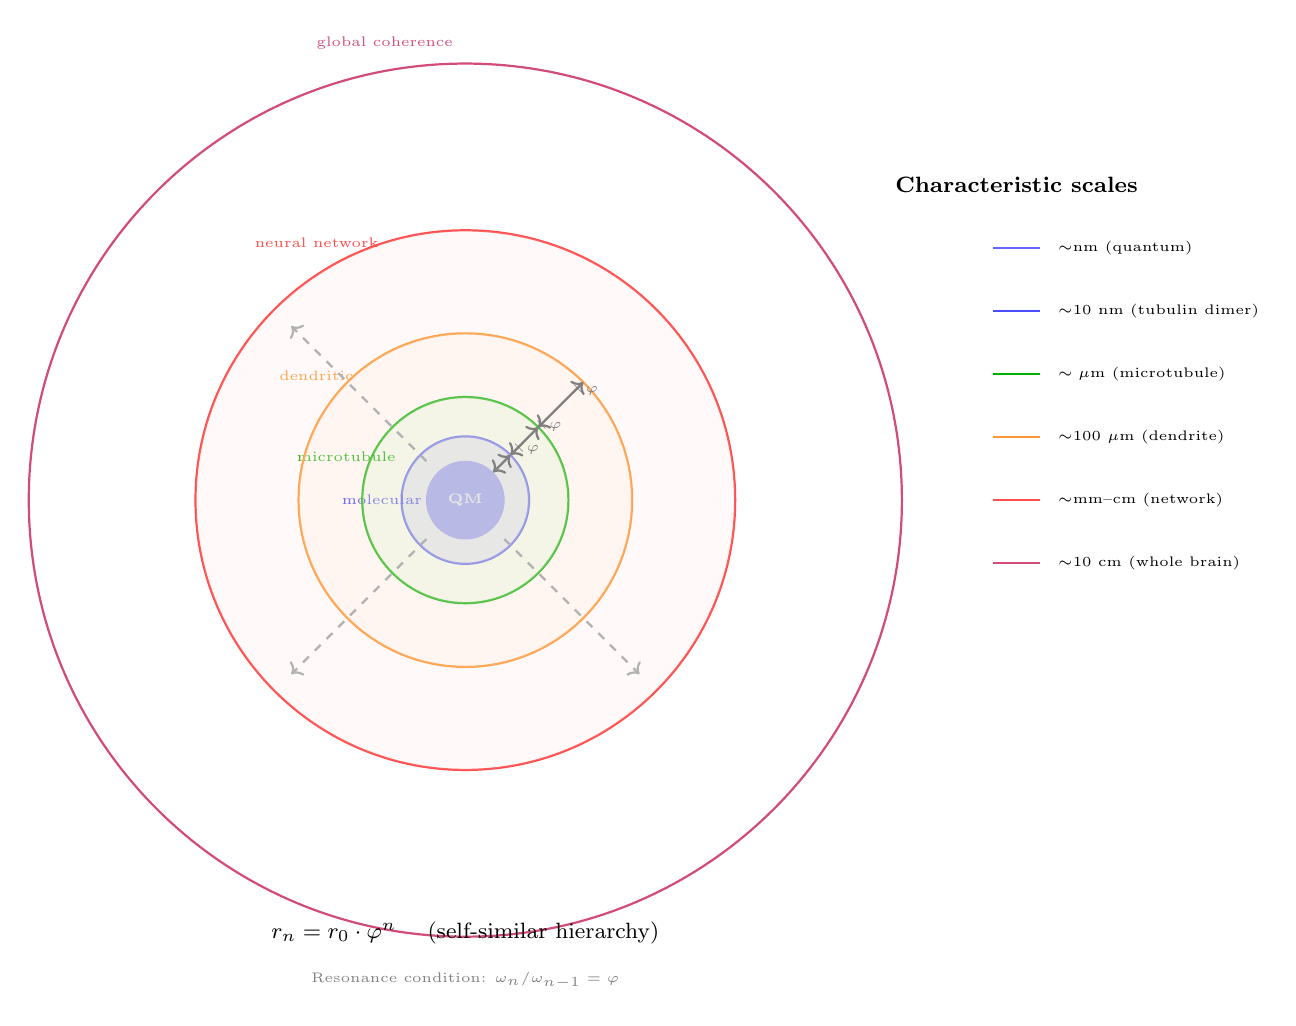
\begin{tikzpicture}[scale=1]

% === Define golden ratio ===
\pgfmathsetmacro{\phi}{1.618}

% === Central quantum core ===
\fill[blue!60,opacity=0.8] (0,0) circle (0.5);
\node[white,font=\tiny\bfseries] at (0,0) {QM};

% === Shell 1: Molecular (tubulin) ===
\pgfmathsetmacro{\rone}{0.5*\phi}
\draw[thick,blue!70] (0,0) circle (\rone);
\fill[blue!30,opacity=0.3] (0,0) circle (\rone);
\node[font=\tiny,blue!80] at (180:\rone+0.25) {molecular};

% === Shell 2: Microtubule ===
\pgfmathsetmacro{\rtwo}{\rone*\phi}
\draw[thick,green!70!black] (0,0) circle (\rtwo);
\fill[green!30,opacity=0.2] (0,0) circle (\rtwo);
\node[font=\tiny,green!70!black] at (160:\rtwo+0.3) {microtubule};

% === Shell 3: Dendritic ===
\pgfmathsetmacro{\rthree}{\rtwo*\phi}
\draw[thick,orange!80] (0,0) circle (\rthree);
\fill[orange!20,opacity=0.2] (0,0) circle (\rthree);
\node[font=\tiny,orange!80] at (140:\rthree+0.35) {dendritic};

% === Shell 4: Neural network ===
\pgfmathsetmacro{\rfour}{\rthree*\phi}
\draw[thick,red!70] (0,0) circle (\rfour);
\fill[red!15,opacity=0.15] (0,0) circle (\rfour);
\node[font=\tiny,red!70] at (120:\rfour+0.35) {neural network};

% === Shell 5: Global brain ===
\pgfmathsetmacro{\rfive}{\rfour*\phi}
\draw[thick,purple!70] (0,0) circle (\rfive);
\node[font=\tiny,purple!70] at (100:\rfive+0.35) {global coherence};

% === Scale labels on right side ===
\begin{scope}[shift={(7,0)}]
    \node[font=\footnotesize\bfseries] at (0,4) {Characteristic scales};

    \draw[blue!60,thick] (-0.3,3.2) -- (0.3,3.2);
    \node[right,font=\tiny] at (0.4,3.2) {$\sim$nm (quantum)};

    \draw[blue!70,thick] (-0.3,2.4) -- (0.3,2.4);
    \node[right,font=\tiny] at (0.4,2.4) {$\sim$10 nm (tubulin dimer)};

    \draw[green!70!black,thick] (-0.3,1.6) -- (0.3,1.6);
    \node[right,font=\tiny] at (0.4,1.6) {$\sim\mu$m (microtubule)};

    \draw[orange!80,thick] (-0.3,0.8) -- (0.3,0.8);
    \node[right,font=\tiny] at (0.4,0.8) {$\sim$100 $\mu$m (dendrite)};

    \draw[red!70,thick] (-0.3,0) -- (0.3,0);
    \node[right,font=\tiny] at (0.4,0) {$\sim$mm--cm (network)};

    \draw[purple!70,thick] (-0.3,-0.8) -- (0.3,-0.8);
    \node[right,font=\tiny] at (0.4,-0.8) {$\sim$10 cm (whole brain)};
\end{scope}

% === Phi-ratio annotation ===
\draw[<->,thick,gray] (45:0.5) -- (45:\rone);
\node[gray,font=\tiny,above right] at (45:{0.5+(\rone-0.5)/2}) {$\times\varphi$};

\draw[<->,thick,gray] (45:\rone) -- (45:\rtwo);
\node[gray,font=\tiny,above right] at (45:{\rone+(\rtwo-\rone)/2}) {$\times\varphi$};

\draw[<->,thick,gray] (45:\rtwo) -- (45:\rthree);
\node[gray,font=\tiny,above right] at (45:{\rtwo+(\rthree-\rtwo)/2}) {$\times\varphi$};

% === Resonance coupling arrows (bidirectional) ===
\foreach \angle in {135,225,315} {
    \draw[->,thick,gray!60,dashed] (\angle:0.7) -- (\angle:\rfour-0.3);
}

% === Caption equation ===
\node[font=\footnotesize] at (0,-5.5) {$r_n = r_0 \cdot \varphi^n$ \quad (self-similar hierarchy)};
\node[font=\tiny,gray] at (0,-6.1) {Resonance condition: $\omega_n / \omega_{n-1} = \varphi$};

\end{tikzpicture}
\end{document}
